%%
%% Copyright (c) 2018-2019 Weitian LI <liweitianux@sjtu.edu.cn>
%% Creative Commons BY 4.0
%%

\chapter{Fokker--Planck 方程数值算法}
\label{app:fpsolver}

在\ac{mfluid}中,带电粒子可与其中的湍流发生随机散射而通过\emph{二阶 Fermi 加速}机制
获得能量\cite{fermi1949,fermi1954,davis1956},
该过程可由 Fokker--Planck 方程描述
\cite{schlickeiser1989,eilek1991,schlickeiser2002}.
当加速区域是均匀的且远大于散射的\ac{mfp}时,Fokker--Planck 方程可被简化到只
依赖于时间和能量\cite{park1995,park1996}:
\begin{equation}
  \label{eq:fp-generic}
  \pdiff{u(x,t)}{t} = \frac{1}{A(x)} \pdiff{}{x}
    \left[ B(x) u(x,t) + C(x) \pdiff{u(x,t)}{x} \right]
    - \frac{u(x,t)}{T(x)} + Q(x) ,
\end{equation}
其中
$x$ 是能量或动量,
$u(x,t)$ 为粒子的能量分布,
$A(x)$ 为相位因子(如果 $x$ 表示能量,该项等于 1;
如果 $x$ 表示动量,该项等于 $4\Cpi x^2$),
$B(x)$、$C(x)$、$T(x)$ 和 $Q(x)$ 分别描述了粒子的
平流 (advection)、扩散 (diffusion)、逃逸 (escape) 和注入 (injection).
这几个系数需满足 $A(x) > 0, C(x) > 0, T(x) \ge 0, Q(x) \ge 0$.

然而,简化后的 Fokker--Planck 方程仍然只能在有限的几种特殊情况下获得解析解,
而对于一般情况则必须求助于数值算法.
由 \citeay{chang1970} 提出的有限差分法 (finite difference scheme)
是一种有效的算法,下文对该算法作具体介绍.


%=====================================================================
\section{数值算法}

采用一个包含 $M+1$ 个点的网格对 $x$ 离散化:$x_m (m = 0, 1, \cdots, M)$.
在网格单元中点处,$x$ 的值定义为:
\begin{equation}
  \label{eq:x-mid}
  x_{m+1/2} = (x_m + x_{m+1}) \big/ 2 ,
\end{equation}
同时 $\Delta x$ 的值定义为:
\begin{equation}
  \label{eq:dx-mid}
  \Delta x_{m+1/2} = x_{m+1} - x_m ,
\end{equation}
于是可得:
\begin{equation}
  \label{eq:dx}
  \Delta x_m = (x_{m+1} - x_{m-1}) \big/ 2 .
\end{equation}
对时间 $t$ 离散化,并采用记法:
\begin{equation}
  \label{eq:u-t}
  u_m^n = u(x_m, t_n) .
\end{equation}

接着,定义 $x$-空间的粒子流量 $F(x,t)$ 为:
\begin{equation}
  \label{eq:fp-f}
  F(x,t) = B(x) u(x,t) + C(x) \pdiff{u(x,t)}{x} .
\end{equation}
于是\emph{无流量 (no-flux) 边界条件}可写为\cite{park1995}:
\begin{equation}
  \label{eq:no-flux}
  F(x_0, t) = F(x_M, t) = 0 .
\end{equation}

对\autoref{eq:fp-generic} 离散化可得:
\begin{equation}
  \label{eq:fp-disc}
  \frac{u_m^{n+1} - u_m^n}{\Delta t}
    = \frac{1}{A_m} \frac{F_{m+1/2}^{n+1} - F_{m-1/2}^{n+1}}{\Delta x_m}
      - \frac{u_m^{n+1}}{T_m} + Q_m ,
\end{equation}
其中 $\Delta t = t_{n+1} - t_n$ 为时间步长.
同时\autoref{eq:no-flux} 的无流量边界条件成为:
\begin{equation}
  \label{eq:no-flux-disc}
  F_{-1/2}^{n+1} = F_{M+1/2}^{n+1} = 0 .
\end{equation}

\citeay{chang1970} 给出如下 $F_{m+1/2}^{n+1}$ 的表达式:
\begin{align}
  \label{eq:fp-f-chang70}
  F_{m+1/2}^{n+1} & = (1 - \delta_{m+1/2}) B_{m+1/2} u_{m+1}^{n+1}
      + \delta_{m+1/2} B_{m+1/2} u_m^{n+1}
      + C_{m+1/2} \frac{u_{m+1}^{n+1} - u_m^{n+1}}{\Delta x_{m+1/2}} \\
    & = \frac{C_{m+1/2}}{\Delta x_{m+1/2}} \left[
      W_{m+1/2}^{+} u_{m+1}^{n+1} - W_{m+1/2}^{-} u_m^{n+1} \right] ,
\end{align}
其中
\begin{align}
  \delta_m & = \frac{1}{w_m} - \frac{1}{\exp(w_m) - 1} ,
    \label{eq:fp-delta-m} \\
  W_m^{\pm} & = W_m \exp(\pm w_m / 2) ,
    \label{eq:fp-Wm-pm} \\
  W_m & = w_m \big/ [2 \sinh(w_m / 2)] ,
    \label{eq:fp-Wm} \\
  w_m & = \frac{B_m}{C_m} \Delta x_m .
    \label{eq:fp-wm}
\end{align}
考虑到 $|w_m|$ 可能会非常大或者非常小,为了使数值计算更稳定,可采用\cite{park1996}:
\begin{equation}
  \label{eq:fp-Wm-calc}
  W_m = \left\{
    \begin{alignedat}{2}
      & \left[ 1 + \frac{w_m^2}{24} + \frac{w_m^4}{1920} \right]^{-1} ,
        & \quad\text{when~} |w_m| < 0.1 , \\
      & \frac{|w_m| \exp(-|w_m|/2)}{1 - \exp(-|w_m|)} ,
        & \quad\text{when~} |w_m| \ge 0.1 .
    \end{alignedat}
  \right.
\end{equation}

将\autoref{eq:fp-f-chang70} 代入\autoref{eq:fp-disc},
可整理成如下三对角 (tridigonal) 线性方程组:
\begin{equation}
  \label{eq:fp-tridigonal}
  \left\{
    \begin{aligned}
      -a_m u_{m-1}^{n+1} + b_m u_m^{n+1} - c_m u_{m+1}^{n+1} & = r_m, \\
      a_0 = c_M & = 0 ,
    \end{aligned}
  \right.
\end{equation}
其中各项系数如下:
\begin{equation}
  \label{eq:fp-coefs}
  \left\{
    \begin{aligned}
      a_m & = \frac{\Delta t}{A_m \Delta x_m}
        \frac{C_{m-1/2}}{\Delta x_{m-1/2}} W_{m-1/2}^{-} , \\
      c_m & = \frac{\Delta t}{A_m \Delta x_m}
        \frac{C_{m+1/2}}{\Delta x_{m+1/2}} W_{m+1/2}^{+} , \\
      b_m & = 1 + \frac{\Delta t}{A_m \Delta x_m}
        \left[ \frac{C_{m-1/2}}{\Delta x_{m-1/2}} W_{m-1/2}^{+}
        + \frac{C_{m+1/2}}{\Delta x_{m+1/2}} W_{m+1/2}^{-} \right]
        + \frac{\Delta t}{T_m} , \\
      r_m & = u_m^n + \Delta t Q_m .
    \end{aligned}
  \right.
\end{equation}
注意,上式无法给出 $b_0$ 和 $b_M$,这需要利用边界条件[\autoref{eq:no-flux-disc}]
重新推导系数,可得:
\begin{equation}
  \label{eq:fp-coefs-b}
  \left\{
    \begin{aligned}
      b_0 & = 1 + \frac{\Delta t}{A_0 \Delta x_0}
        \frac{C_{1/2}}{\Delta x_{1/2}} W_{1/2}^{-}
        + \frac{\Delta t}{T_0} , \\
      b_M & = 1 + \frac{\Delta t}{A_M \Delta x_M}
        \frac{C_{M-1/2}}{\Delta x_{M-1/2}} W_{M-1/2}^{+}
        + \frac{\Delta t}{T_M} .
    \end{aligned}
  \right.
\end{equation}
\autoref{eq:fp-tridigonal} 的线性方程组可由快速的三对角矩阵算法
(亦称 Thomas 算法)求解\cite{press1992}.

在无流量边界条件下,粒子可能在边界处堆积,这对本文所研究的湍流加速应用来说是不合理的,
因此需要在边界处进行额外处理.
可在边界处选定一个\enquote{缓冲区},在每个时间步,利用缓冲区外的有效粒子能谱,
按幂律谱外延并替换缓冲区内的能谱\cite{borovsky1986,donnert2014}.


%=====================================================================
\section{算法测试}

为了检测算法的实现是否正确,可将其应用于几种已知解析解的情况\cite{park1996,donnert2014}.
第一个测试是\emph{硬球公式 (hard-sphere equation)}%
\footnote{\citeay{park1996} 的公式 (22) 和 \citeay{donnert2014} 的公式 (34)
均写错了一个正负号.}:
\begin{equation}
  \label{eq:fp-test1}
  \pdiff{u}{t} = \pdiff{}{x} \left[ x^2 \pdiff{u}{x} + (1-x) u \right]
    - u + \delta(x-x_{\R{inj}}) \Theta(t) ,
\end{equation}
其中 $x_{\R{inj}} = 0.1$ 为注入粒子的能量值,
$\Theta(t)$ 为 Heaviside 阶跃函数 (step function).
此例可用于测试算法能否有效处理 $B(x)$ 跨越多个数量级的情况.

第二个测试是:
\begin{equation}
  \label{eq:fp-test2}
  \pdiff{u}{t} = \pdiff{}{x} \left[ x^2 \pdiff{u}{x} - x u \right]
    - \frac{u}{x} + \delta(x-x_{\R{inj}}) \Theta(t) .
\end{equation}
相比第一个测试,此测试中的逃逸项 $T(x)$ 增加了能量依赖而具有多个数量级的变化.

第三个测试是:
\begin{equation}
  \label{eq:fp-test3}
  \pdiff{u}{t} = \pdiff{}{x} \left[ x^3 \pdiff{u}{x} - x^2 u \right]
    - u + \delta(x-x_{\R{inj}}) \delta(t) .
\end{equation}
此例用于测试算法的时间演化准确度.

我们选取了对数网格,将 $x \in [\num{e-4}, \num{e4}]$ 划分为 $M=200$ 个单元,
时间步长固定为 $\Delta t = \num{e-3}$,
求解以上三个测试,结果如\autoref{fig:fp-test12} 和\autoref{fig:fp-test3} 所示.
我们的结果与 \citeay{park1996} 以及 \citeay{donnert2014} 的结果非常吻合,
说明我们的算法实现是正确可靠的.

\begin{figure}[htp]
  \centering
  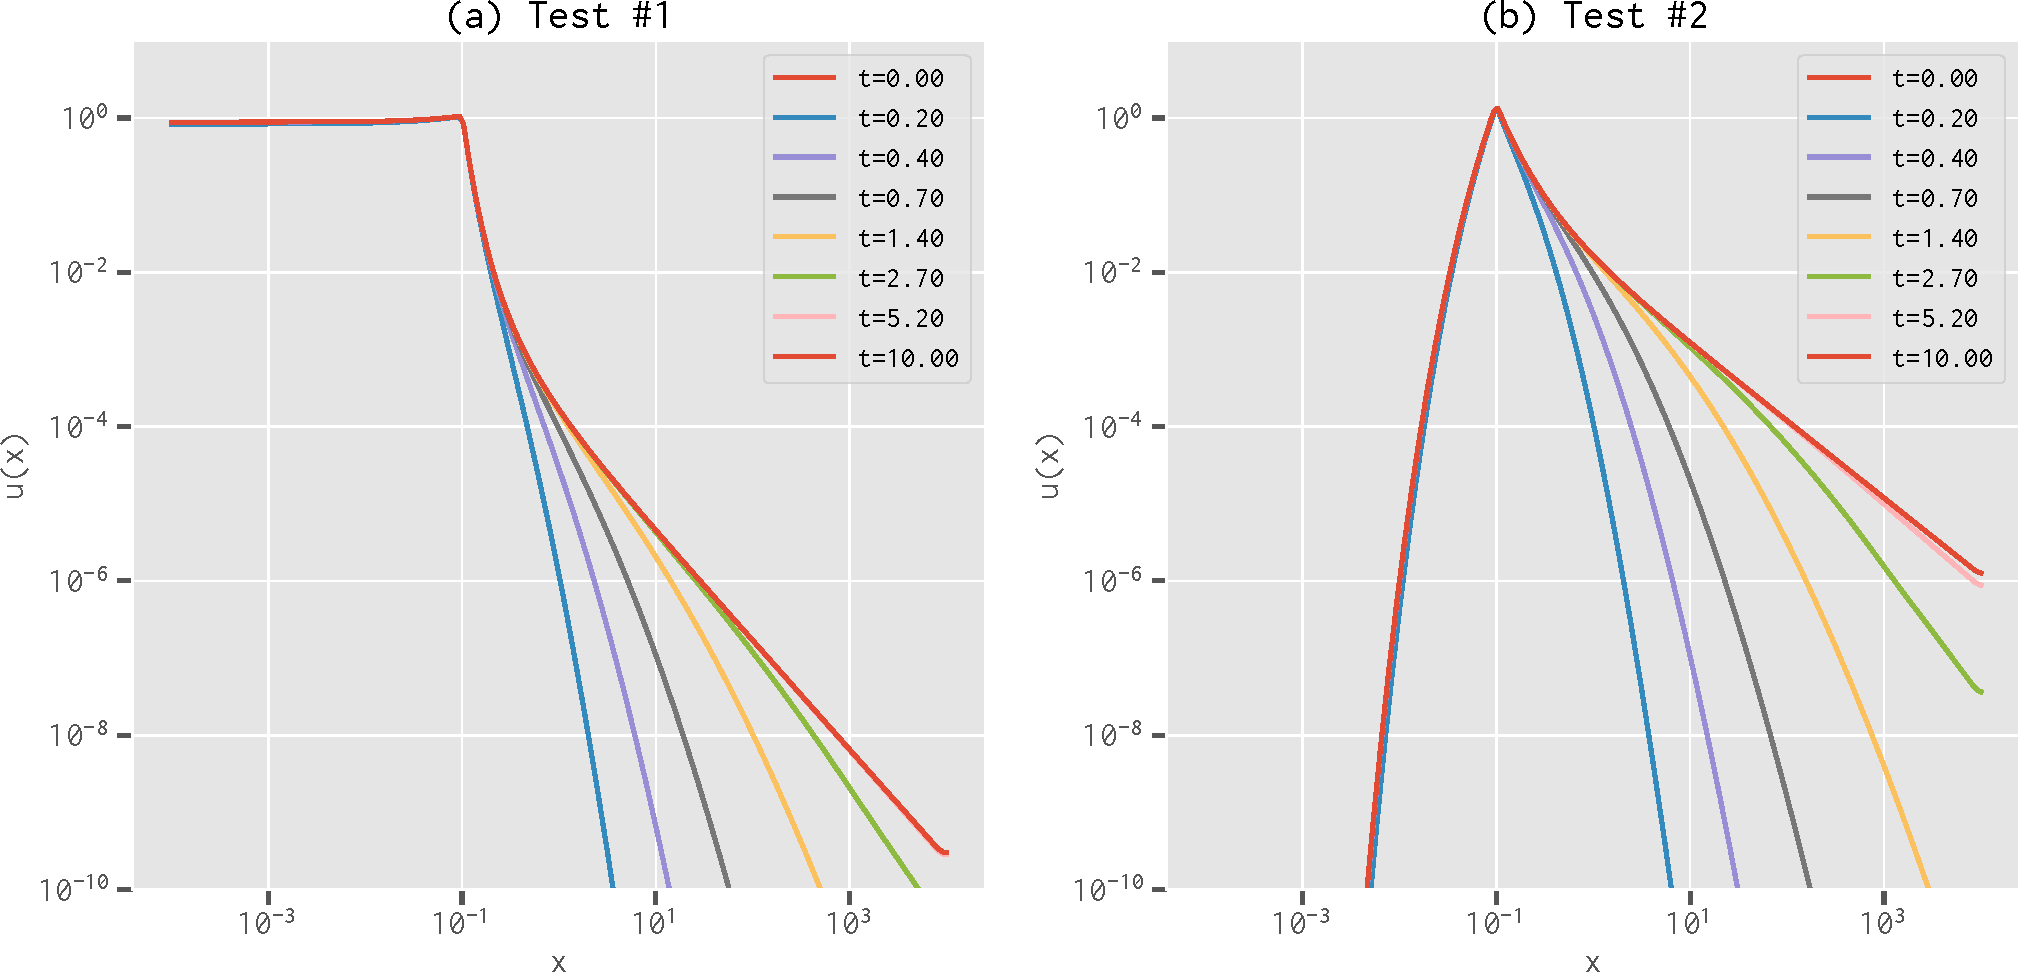
\includegraphics[width=\textwidth]{fp-test12}
  \bicaption[Fokker--Planck 方程算法测试 (1 \& 2)]{%
    Fokker--Planck 方程算法测试 (1 \& 2).
    左栏和右栏分别显示了求解第一个测试 [\autoref{eq:fp-test1}]
    和第二个测试 [\autoref{eq:fp-test2}] 获得的粒子能谱.
  }{%
    Testing of the implementation of the Fokker--Planck equation
    solver.
    The left and right panels represent the derived particle spectra
    for the first test [Eq.~\ref{eq:fp-test1}] and
    the second test [Eq.~\ref{eq:fp-test2}], respectively.
  }
  \label{fig:fp-test12}
\end{figure}

\begin{figure}[htp]
  \centering
  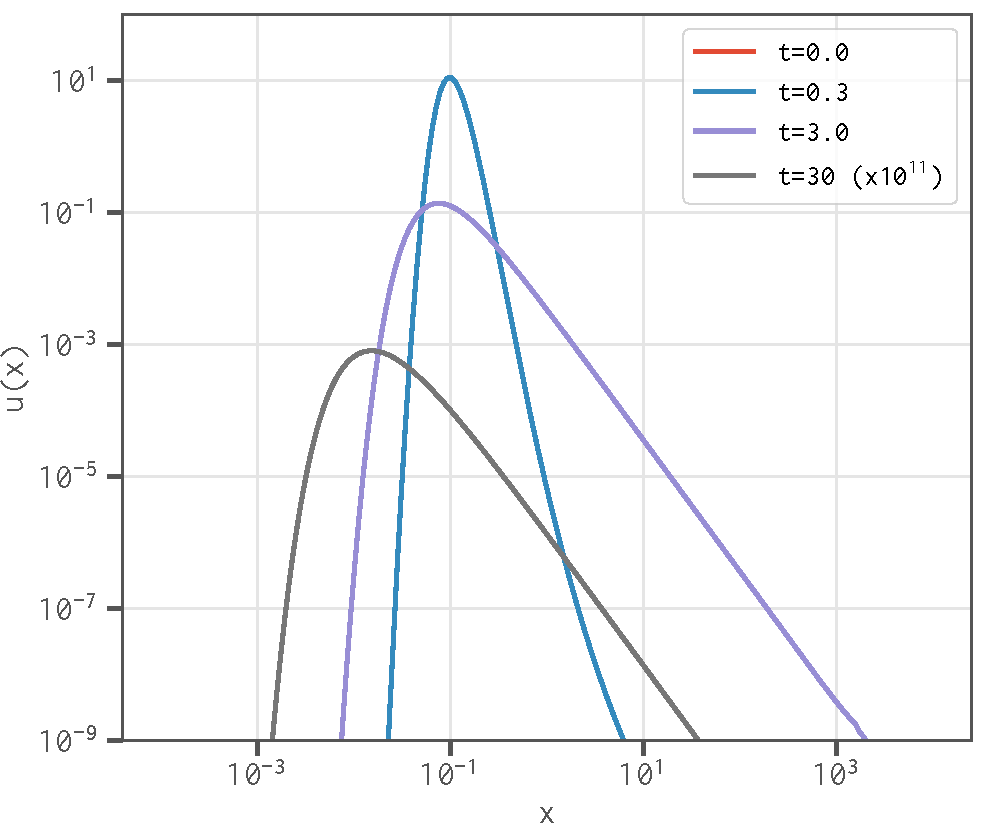
\includegraphics[width=0.55\textwidth]{fp-test3}
  \bicaption[Fokker--Planck 方程算法测试 (3)]{%
    Fokker--Planck 方程算法测试 (3).
    求解第三个测试 [\autoref{eq:fp-test3}] 获得的粒子能谱.
    注意 $t = 30$ 对应的能谱已乘了 \num{e11} 以更好地显示.
  }{%
    The derived particle spectra for the third test [Eq.~\ref{eq:fp-test2}].
    Note that the spectrum of $t = 30$ has been multiplied by \num{e11}
    for clarity.
  }
  \label{fig:fp-test3}
\end{figure}


%% EOF
